\documentclass[aspectratio=169,10pt]{beamer}

\usepackage{amsmath,amssymb}
\usepackage{booktabs}
\usepackage{array}
\usepackage{tikz}
\usepackage{graphicx}
\usepackage{hyperref}
\usetikzlibrary{arrows.meta,positioning,shapes.geometric,calc}

\usetheme{default}

% ---------------------------------------------------------
% COLOR PALETTE
% ---------------------------------------------------------
\definecolor{Navy}{RGB}{20,38,65}
\definecolor{Blue}{RGB}{38,90,155}
\definecolor{Teal}{RGB}{28,125,130}
\definecolor{AccentGreen}{RGB}{34,160,110}
\definecolor{DarkGray}{RGB}{50,55,60}
\definecolor{MediumGray}{RGB}{100,105,112}
\definecolor{LightGray}{RGB}{245,247,250}
\definecolor{LightBlue}{RGB}{235,243,252}
\definecolor{LightTeal}{RGB}{232,246,246}
\definecolor{LightAmber}{RGB}{254,245,232}

% ---------------------------------------------------------
% BEAMER STYLING
% ---------------------------------------------------------
\setbeamertemplate{navigation symbols}{}
\setbeamersize{text margin left=0.6cm,text margin right=0.6cm}

\setbeamercolor{normal text}{fg=DarkGray,bg=white}
\setbeamercolor{structure}{fg=Blue}
\setbeamercolor{frametitle}{fg=white,bg=Navy}
\setbeamerfont{frametitle}{size=\large,series=\bfseries}

\setbeamertemplate{frametitle}{%
  \nointerlineskip%
  \begin{beamercolorbox}[wd=\paperwidth,ht=0.82cm,dp=0.18cm,leftskip=0.6cm]{frametitle}%
    \usebeamerfont{frametitle}\insertframetitle%
  \end{beamercolorbox}%
}

\setbeamertemplate{footline}{%
  \leavevmode%
  \hbox{%
    \begin{beamercolorbox}[wd=.75\paperwidth,ht=0.28cm,dp=0.08cm,leftskip=0.6cm]{author in head/foot}%
      \color{MediumGray}\scriptsize EV Charging Infrastructure Optimization \quad$\vert$\quad Group D07%
    \end{beamercolorbox}%
    \begin{beamercolorbox}[wd=.25\paperwidth,ht=0.28cm,dp=0.08cm,rightskip=0.6cm]{author in head/foot}%
      \color{MediumGray}\scriptsize\hfill\insertframenumber\,/\,\inserttotalframenumber%
    \end{beamercolorbox}%
  }%
}

\setbeamertemplate{itemize item}{\color{Teal}\small$\blacktriangleright$}
\setbeamertemplate{itemize subitem}{\color{Blue}\tiny$\bullet$}

% =========================================================
% DOCUMENT BEGINS
% =========================================================
\begin{document}

% ---------------------------------------------------------
% SLIDE 1: TITLE PAGE (AS REQUESTED)
% ---------------------------------------------------------
\begin{frame}[plain]

\vspace{0.65cm}

\begin{columns}[c]

% =========================================================
% Vertical accent line
% =========================================================
\begin{column}{0.06\textwidth}

\begin{tikzpicture}
\fill[Teal] (0,0) rectangle (0.16,5.0);
\end{tikzpicture}
\end{column}

% =========================================================
% Main content
% =========================================================
\begin{column}{0.88\textwidth}

% Title
{\fontsize{24}{29}\selectfont
\color{Navy}
\textbf{EV Charging Infrastructure Optimization}}\\[-1mm]

\vspace{0.55cm}

% Group number
{\large
\textbf{Group Number:} \color{Teal}\textbf{D07}
}

\vspace{0.35cm}

% Group members heading
{\large
\color{Navy}
\textbf{Group Members:}
}

\vspace{0.18cm}

% Members
{\normalsize
\textbf{Rishi Raajha A} -- CB.SC.U4AIE23335\\[1.5mm]
\textbf{Harshvardhan V} -- CB.SC.U4AIE23353\\[1.5mm]
\textbf{Naveen Sankar R S} -- CB.SC.U4AIE23323\\[1.5mm]
\textbf{Sakthi Pranav S} -- CB.SC.U4AIE23336
}

\end{column}

\end{columns}

\end{frame}

% ---------------------------------------------------------
% SLIDE 2: INTRODUCTION (5 SINGLE-LINE POINTS)
% ---------------------------------------------------------
\begin{frame}{Introduction}
  \vspace{0.35cm}
  \begin{itemize}\setlength{\itemsep}{0.45cm}
    \item Rapid global adoption of Electric Vehicles demands a scalable and capital-efficient expansion of public charging infrastructure.
    \item Unplanned commercial deployments lead to dense urban clustering while leaving vital highway transit corridors as charging deserts.
    \item Current physical charging infrastructure growth lags significantly behind the exponential surge in global EV adoption.
    \item Ad-hoc planning heuristics fail to balance commercial facility accessibility with public regional equity under fixed capital budgets.
    \item We formulate an exact Operations Research framework to optimize strategic corridor hub siting alongside fair territorial resource allocation.
  \end{itemize}
\end{frame}



% ---------------------------------------------------------
% SLIDE 4: DATASET DESCRIPTION - GENERAL DETAILS
% ---------------------------------------------------------
\begin{frame}{Dataset Description}
  \vspace{0.1cm}
  \begin{itemize}\setlength{\itemsep}{0.12cm}
    \item \textbf{Data Origin:} OpenChargeMap public global charging station registry (\textit{risheepanchal/global-ev-charging-stations-dataset}).
    \item \textbf{Record Universe:} 10,000 total records across 30+ countries in North America, Europe, Asia, and Australasia.
    \item \textbf{Operational Universe:} Exactly \textbf{9,301 active stations} after filtering out 312 offline and 387 planned/unknown records.
  \end{itemize}
  \vspace{0.15cm}
  \begin{table}[h]
    \centering
    \scriptsize
    \renewcommand{\arraystretch}{1.2}
    \begin{tabular}{p{2.5cm}p{1.8cm}p{4.2cm}p{4.2cm}}
      \toprule
      \textbf{Attribute} & \textbf{Data Type} & \textbf{Description} & \textbf{Role in Optimization} \\
      \midrule
      \texttt{lat}, \texttt{lon} & Float & WGS84 geographic coordinates & Great-circle Haversine distances \& 3D spherical clustering \\
      \texttt{status} & String & Operational status verification flag & Filters working network ($N = 9,301$) \\
      \texttt{num\_connectors} & Integer & Number of physical charging ports & Baseline regional capacity $C_r$ and CPS computation \\
      \texttt{state} & String & Administrative region / state code & Regional boundaries for equity allocation ($R = 403$) \\
      \texttt{country} & String & ISO 2-letter sovereign code & National and global scoping ($R = 415$ composite) \\
      \bottomrule
    \end{tabular}
  \end{table}
\end{frame}

% ---------------------------------------------------------
% SLIDE 5: DATASET DESCRIPTION - EDA INSIGHTS
% ---------------------------------------------------------
\begin{frame}{Dataset Description: Exploratory Data Analysis}
  \vspace{0.25cm}
  \begin{itemize}\setlength{\itemsep}{0.35cm}
    \item \textbf{The Single-Plug Majority Vulnerability:}
      \begin{itemize}\setlength{\itemsep}{0.12cm}
        \item Over \textbf{52\% of stations operate with only 1 connector}; over 78\% have $\le 2$ connectors.
        \item Single-plug stations offer zero hardware redundancy; an occupied charger or maintenance fault creates total driver stranding.
      \end{itemize}
    \item \textbf{Extreme Geographic Skew:}
      \begin{itemize}\setlength{\itemsep}{0.12cm}
        \item Over 64\% of stations are concentrated in North America (Canada: 3,970, US: 2,099), followed by Western Europe (Spain: 726).
        \item Intercity and highway transit routes remain sparsely served, requiring deliberate regional corridor planning.
      \end{itemize}
    \item \textbf{Administrative Gaps \& Zero-Connector Anomalies:}
      \begin{itemize}\setlength{\itemsep}{0.12cm}
        \item Exactly 5 stations record 0 connectors, reducing the baseline network-wide minimum CPS floor to \textbf{0.0000}.
        \item 2,869 records lack sub-national state values, requiring explicit data handling for administrative equity models.
      \end{itemize}
  \end{itemize}
\end{frame}

% ---------------------------------------------------------
% SLIDE 6: PROBLEM STATEMENT (POINTS, NOT QUESTIONS)
% ---------------------------------------------------------
\begin{frame}{Problem Statement}
  \vspace{0.35cm}
  \begin{itemize}\setlength{\itemsep}{0.42cm}
    \item \textbf{Corridor Coverage Deficits:} Existing charging networks are reactively clustered in high-density urban centers, leaving intercity highway corridors with extensive coverage deserts and no regional fast-charging anchors.
    \item \textbf{Hardware Fragility \& Bottlenecks:} Over 52\% of existing stations operate with only a single connector, offering zero physical redundancy and creating severe driver stranding risks during equipment outages.
    \item \textbf{Systemic Territorial Inequity:} Conventional market-driven and proportional funding mechanisms disproportionately reward already-saturated regions, trapping secondary administrative territories at near-zero charging ratios.
    \item \textbf{Prohibitive Greenfield Capital Barriers:} Building new charging sites from scratch incurs massive land acquisition costs, permitting delays, and grid connection bottlenecks, necessitating strategic brownfield upgrading.
  \end{itemize}
\end{frame}


% ---------------------------------------------------------
% SLIDE 7: METHODOLOGY FLOW
% ---------------------------------------------------------
\begin{frame}{Methodology}
  \vspace{0.15cm}
  \begin{center}
    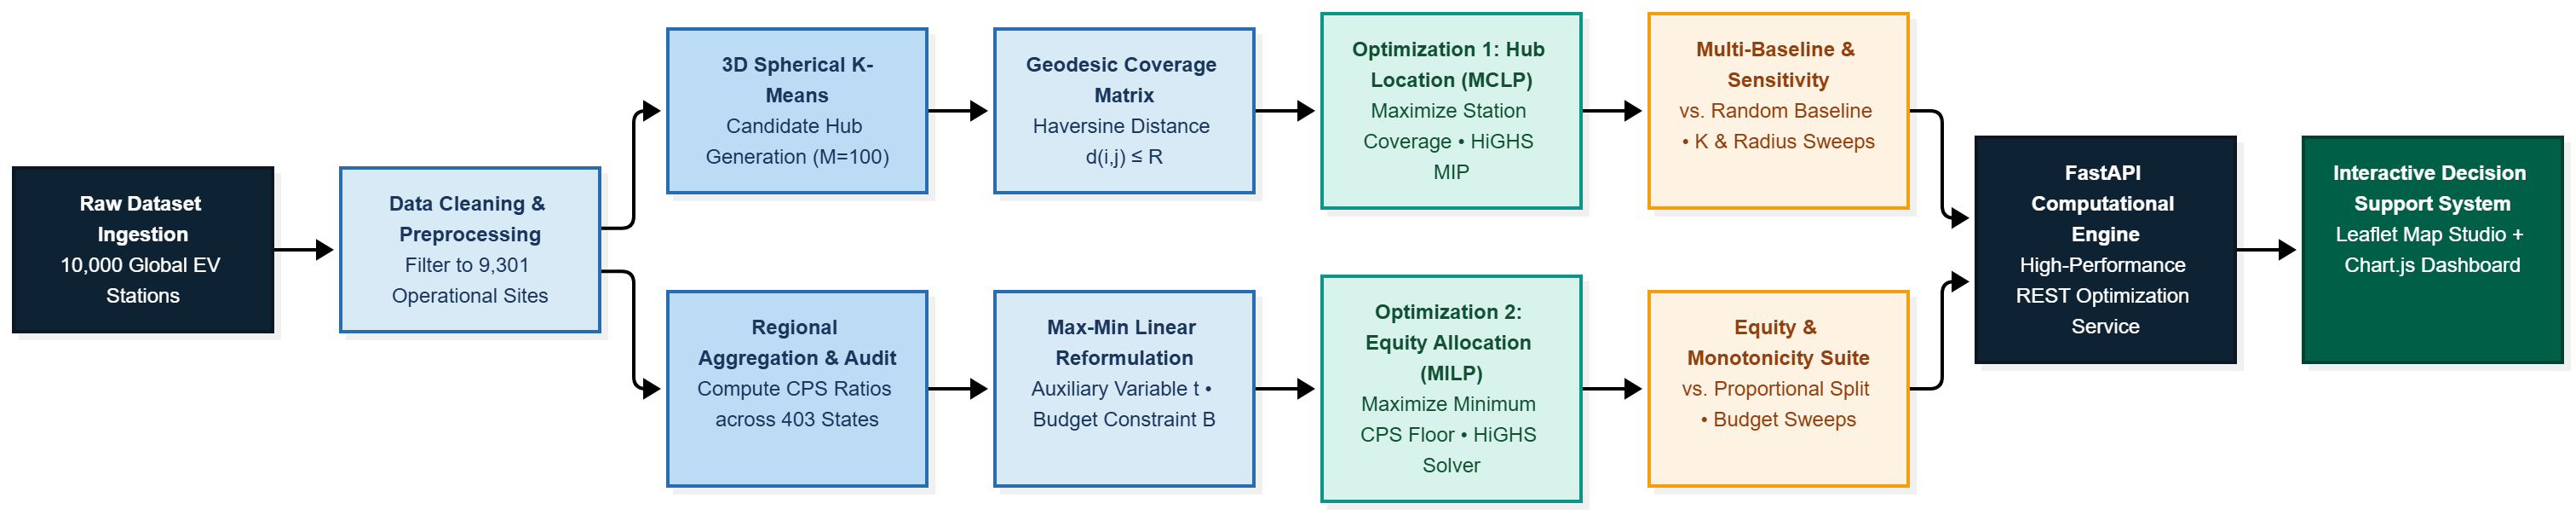
\includegraphics[width=0.98\textwidth,height=0.46\textheight,keepaspectratio]{images/methodology.png}
  \end{center}
\end{frame}

% ---------------------------------------------------------
% SLIDE 8: OPTIMIZATION 1 - CONCEPT
% ---------------------------------------------------------
\begin{frame}{Optimization 1: Strategic Charging Hub Location}
  \vspace{0.15cm}
  \begin{columns}[T]
    \begin{column}{0.48\textwidth}
      \textbf{\color{Navy}Problem Definition \& Brownfield Upgrading}
      \begin{itemize}\setlength{\itemsep}{0.18cm}
        \item \textbf{OR Class:} \textbf{Maximum Covering Location Problem (MCLP)}, Mixed-Integer Programming.
        \item \textbf{What is a Hub?} A high-throughput charging facility with multiple fast plugs serving as a reliable regional anchor.
        \item \textbf{Why Build Hubs?} 52\% of stations have only 1 connector; a 50 km hub provides essential backup during outages or queues.
        \item \textbf{Brownfield Upgrading:} Upgrading existing stations utilizes pre-existing grid interconnects, road access, and permits, saving millions in capital.
      \end{itemize}
    \end{column}
    \begin{column}{0.48\textwidth}
      \textbf{\color{Teal}Role of Spherical K-Means}
      \begin{itemize}\setlength{\itemsep}{0.18cm}
        \item \textbf{Planar Distortion:} Standard 2D K-means distorts distances near higher latitudes as meridians converge.
        \item \textbf{3D Geodesic Preservation:} Projects $(\text{lat}, \text{lon})$ onto a 3D unit sphere to preserve true great-circle Earth geometry.
        \item \textbf{Observed Site Anchoring:} Centroids are snapped to the nearest observed station, guaranteeing roadway and utility feasibility.
      \end{itemize}
    \end{column}
  \end{columns}
\end{frame}

% ---------------------------------------------------------
% SLIDE 9: OPTIMIZATION 1 - FORMULATION
% ---------------------------------------------------------
\begin{frame}{Optimization 1: Mathematical Formulation}
  \vspace{0.15cm}
  \begin{columns}[T]
    \begin{column}{0.50\textwidth}
      \textbf{\color{Navy}MCLP Optimization Model}
      $$\max_{y, z} \quad Z = \sum_{i=1}^{N} z_i$$
      \textbf{Subject to:}
      \begin{align*}
        \sum_{j=1}^{M} y_j &\le K && \text{(Hub Budget)} \\
        z_i &\le \sum_{j \in \mathcal{N}_i} y_j && \forall i \in \{1,\dots,N\} \\
        y_j &\in \{0, 1\} && \forall j \in \{1,\dots,M\} \\
        0 &\le z_i \le 1 && \forall i \in \{1,\dots,N\}
      \end{align*}
      {\scriptsize Where $\mathcal{N}_i = \{j \in \mathcal{J} \mid d(i, j) \le R\}$ is candidate neighborhood.}
    \end{column}
    \begin{column}{0.48\textwidth}
      \textbf{\color{Blue}Variables \& Integrality Property}
      \begin{itemize}\setlength{\itemsep}{0.15cm}
        \item \textbf{Decision Variables:}
          \begin{itemize}\setlength{\itemsep}{0.08cm}
            \item $y_j \in \{0, 1\}$: Binary, 1 if candidate $j$ is established as a hub.
            \item $z_i \in [0, 1]$: Continuous indicator, 1 if station $i$ is covered.
          \end{itemize}
        \item \textbf{Natural Integrality Proof:}
          \begin{itemize}\setlength{\itemsep}{0.08cm}
            \item If no adjacent hub is selected ($\sum y_j = 0$), $z_i \le 0 \implies z_i^* = 0$.
            \item If an adjacent hub is selected ($\sum y_j \ge 1$), $z_i$ pushes to bound $1$.
            \item Basic optimal solutions are naturally integer $\{0, 1\}$; relaxing $z_i$ accelerates solve time by $>100\times$.
          \end{itemize}
      \end{itemize}
    \end{column}
  \end{columns}
\end{frame}

% ---------------------------------------------------------
% SLIDE 10: OPTIMIZATION 2 - CONCEPT
% ---------------------------------------------------------
\begin{frame}{Optimization 2: Regional Connector Allocation}
  \vspace{0.15cm}
  \begin{columns}[T]
    \begin{column}{0.48\textwidth}
      \textbf{\color{Navy}Why Allocate Connectors if Upgrading Hubs?}
      \begin{itemize}\setlength{\itemsep}{0.18cm}
        \item \textbf{Efficiency vs. Equity Duality:} Hub siting (Opt 1) clusters capital in dense traffic corridors; connector allocation (Opt 2) protects peripheral regions.
        \item \textbf{Preventing Neglect:} Market-driven deployment leaves rural and lower-density jurisdictions as charging deserts.
        \item \textbf{Regulatory Mandate:} Directs funding to underserved regions to guarantee territorial baseline parity.
      \end{itemize}
    \end{column}
    \begin{column}{0.48\textwidth}
      \textbf{\color{Teal}Connectors-to-Stations (CPS) Floor}
      \begin{itemize}\setlength{\itemsep}{0.18cm}
        \item \textbf{OR Class:} \textbf{Max-Min Fair Resource Allocation} (Bottleneck MILP / Egalitarian Social Welfare).
        \item \textbf{Target Metric (CPS):} Post-allocation ratio $\text{CPS}_r = \frac{C_r + x_r}{S_r}$ for region $r$.
        \item \textbf{Maximizing the Weakest Link:} Rather than maximizing total connectors (which favors already-dense states), we maximize the minimum floor $t$, elevating the lowest regions.
      \end{itemize}
    \end{column}
  \end{columns}
\end{frame}

% ---------------------------------------------------------
% SLIDE 11: OPTIMIZATION 2 - FORMULATION
% ---------------------------------------------------------
\begin{frame}{Optimization 2: Mathematical Formulation}
  \vspace{0.15cm}
  \begin{columns}[T]
    \begin{column}{0.50\textwidth}
      \textbf{\color{Navy}Max-Min Fair Allocation Model}
      $$\max_{x, t} \quad t$$
      \textbf{Subject to:}
      \begin{align*}
        C_r + x_r &\ge t \cdot S_r && \forall r \in \{1,\dots,R\} \\
        \sum_{r=1}^{R} x_r &\le B && \text{(Connector Budget)} \\
        x_r &\in \mathbb{Z}_{\ge 0} && \forall r \in \{1,\dots,R\} \\
        t &\ge 0 && \text{(Guaranteed Floor)}
      \end{align*}
      {\scriptsize Where $C_r$ is existing connectors, $S_r$ is stations, and $B$ is budget.}
    \end{column}
    \begin{column}{0.48\textwidth}
      \textbf{\color{Blue}Variables \& Linearization}
      \begin{itemize}\setlength{\itemsep}{0.15cm}
        \item \textbf{Decision Variables:}
          \begin{itemize}\setlength{\itemsep}{0.08cm}
            \item $x_r \in \{0, 1, 2,\dots\}$: Integer plugs allocated to region $r$.
            \item $t \ge 0$: Guaranteed minimum regional CPS floor.
          \end{itemize}
        \item \textbf{Linearization Advantage:}
          \begin{itemize}\setlength{\itemsep}{0.08cm}
            \item The non-linear ratio $\frac{C_r + x_r}{S_r} \ge t$ is rearranged into exact linear form $C_r + x_r \ge t \cdot S_r$.
            \item Solved via HiGHS Branch-and-Cut in $<0.05\text{s}$ with guaranteed 0.00\% optimality gap.
            \item Strictly enforces physical integrality (no fractional plugs).
          \end{itemize}
      \end{itemize}
    \end{column}
  \end{columns}
\end{frame}

% ---------------------------------------------------------
% SLIDE 14: RESULTS - OPTIMIZATION 1 SCENARIO
% ---------------------------------------------------------
\begin{frame}{Results: Optimization 1 Benchmark Scenario}
  \begin{columns}[c]
    \begin{column}{0.62\textwidth}
      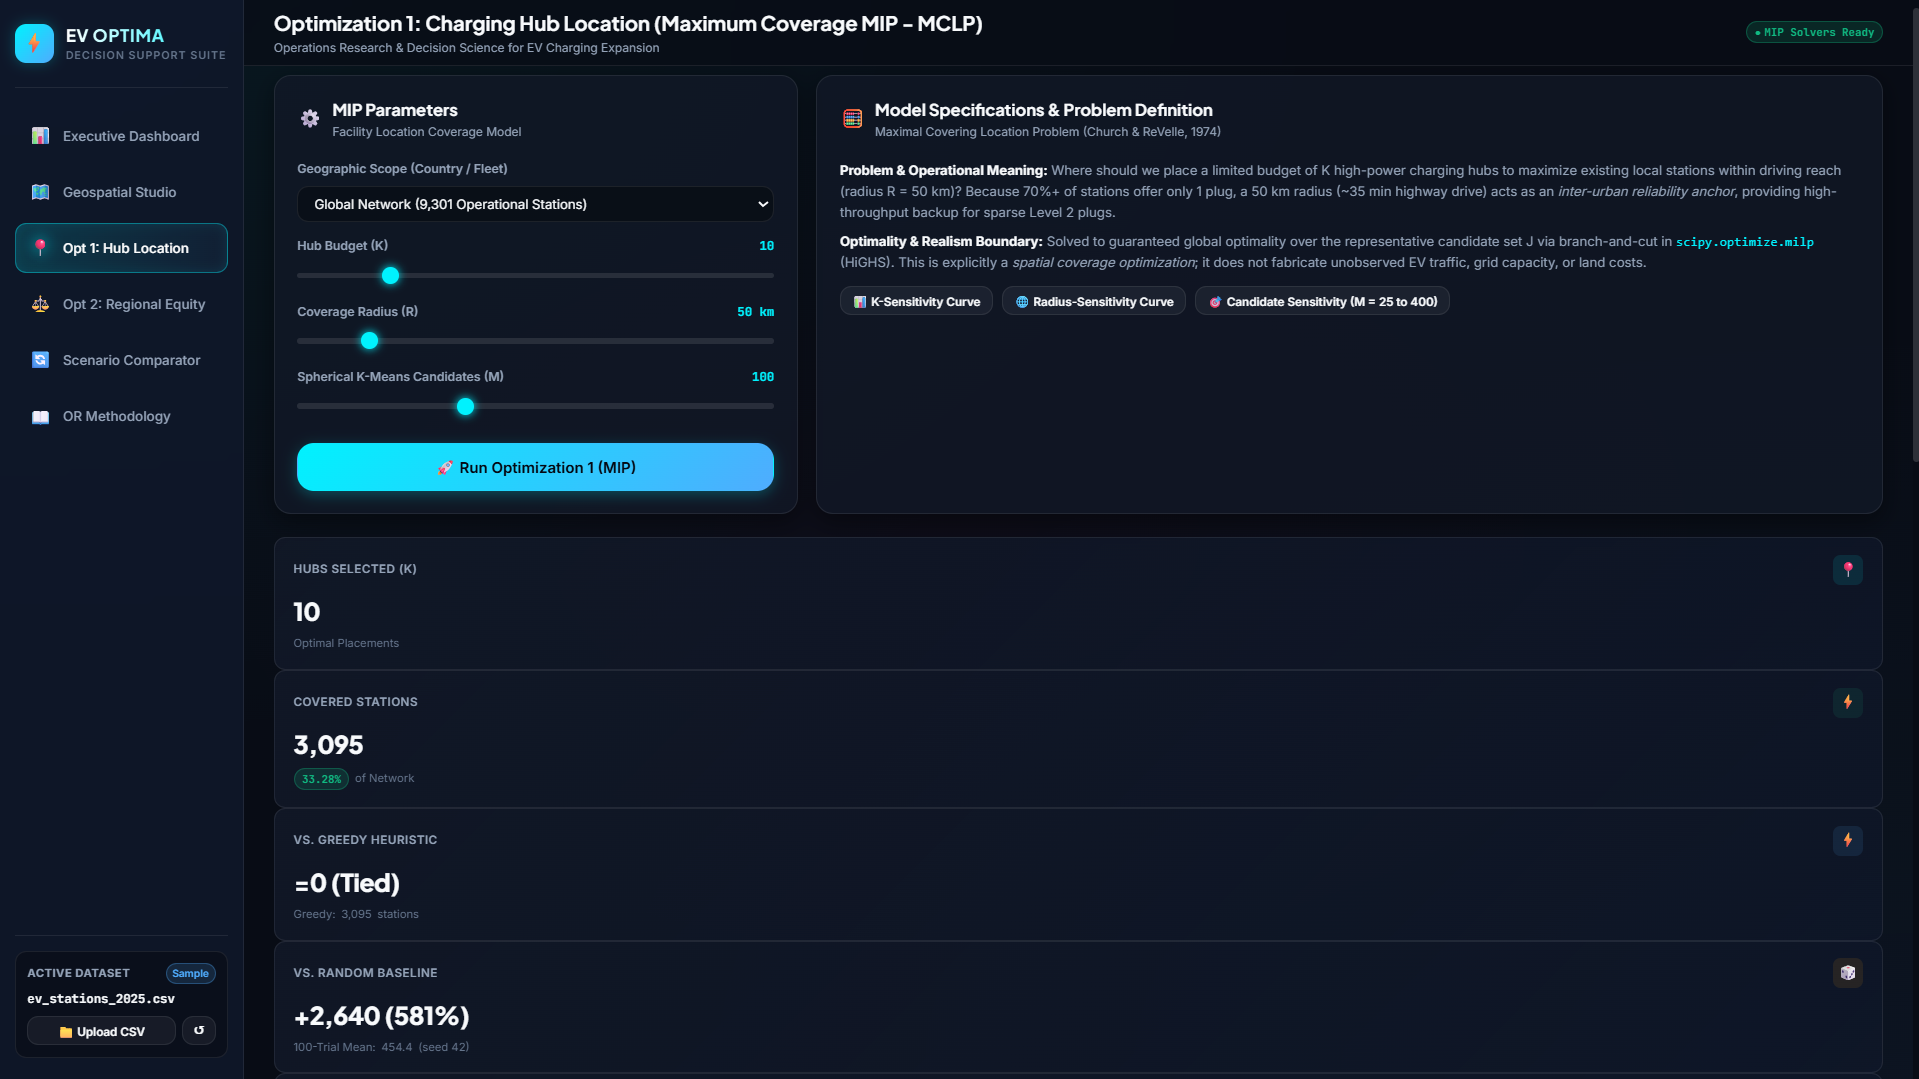
\includegraphics[width=\textwidth,height=0.82\textheight,keepaspectratio]{images/Optimization1.png}
    \end{column}
    \begin{column}{0.36\textwidth}
      \textbf{\color{Navy}Benchmark Solution Metrics}
      \begin{itemize}\setlength{\itemsep}{0.16cm}
        \item \textbf{Parameters:} $K = 10\text{ hubs}$, $R = 50\text{ km}$, $M = 100\text{ candidates}$.
        \item \textbf{High Coverage:} \textbf{3,095 stations (33.28\%)} of the global network covered.
        \item \textbf{Proven Optimality:} Certified \textbf{0.00\% gap} via HiGHS Branch-and-Cut ($<0.15\text{s}$).
        \item \textbf{vs. Random Placement:} \textbf{+581\% advantage} ($Z = 15.94\sigma$ over random mean of 454.4).
      \end{itemize}
    \end{column}
  \end{columns}
\end{frame}

% ---------------------------------------------------------
% SLIDE 15: RESULTS - OPTIMIZATION 1 HUB MAPPING
% ---------------------------------------------------------
\begin{frame}{Results: Charging Hub Geospatial Siting}
  \begin{columns}[c]
    \begin{column}{0.62\textwidth}
      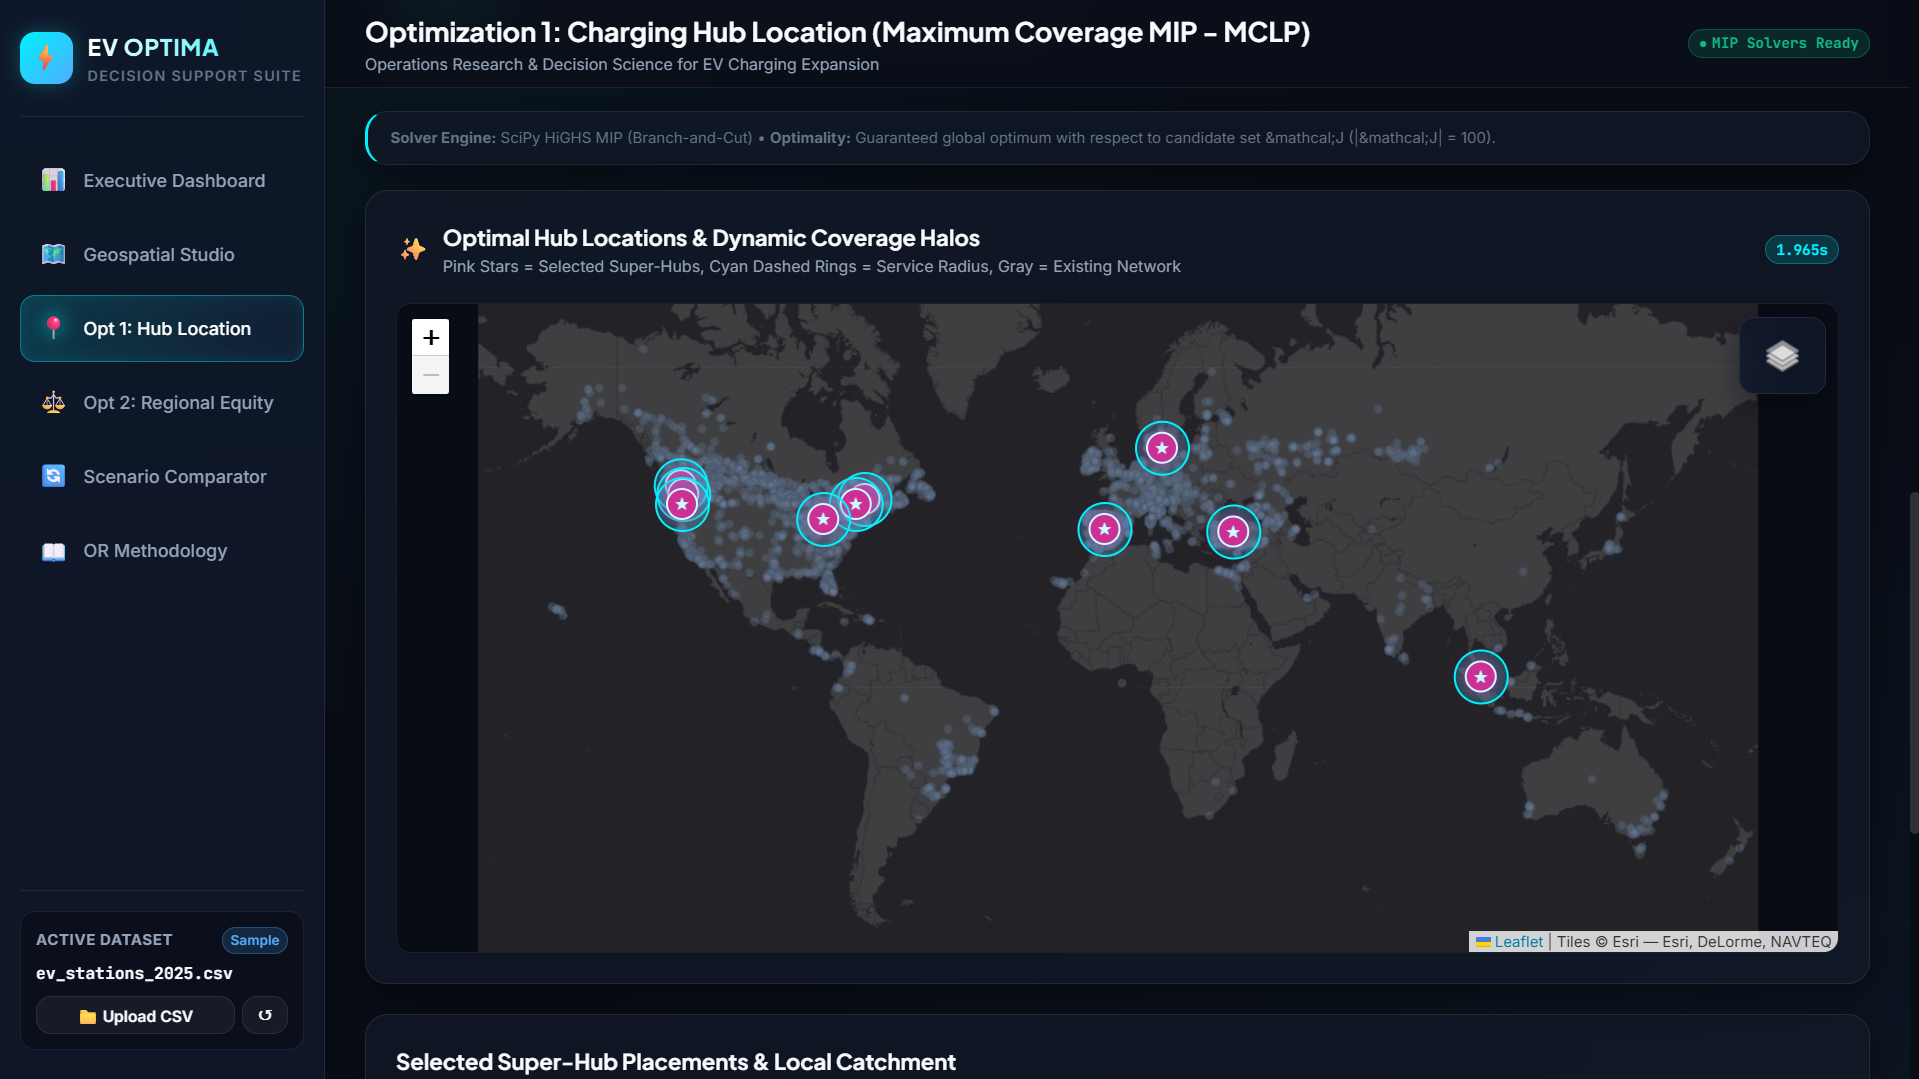
\includegraphics[width=\textwidth,height=0.82\textheight,keepaspectratio]{images/Optimization1_Hubs.png}
    \end{column}
    \begin{column}{0.36\textwidth}
      \textbf{\color{Blue}Hub Placement Takeaways}
      \begin{itemize}\setlength{\itemsep}{0.18cm}
        \item \textbf{Corridor Anchors:} 10 hubs placed at high-density highway transit junctions.
        \item \textbf{50 km Safety Canopies:} Circular buffers protect neighboring 1-plug stations.
        \item \textbf{Brownfield Sites:} Every hub is placed at an existing station with confirmed road and grid access.
      \end{itemize}
    \end{column}
  \end{columns}
\end{frame}

% ---------------------------------------------------------
% SLIDE 16: RESULTS - OPTIMIZATION 2 SCENARIO
% ---------------------------------------------------------
\begin{frame}{Results: Optimization 2 Equity Scenario}
  \begin{columns}[c]
    \begin{column}{0.62\textwidth}
      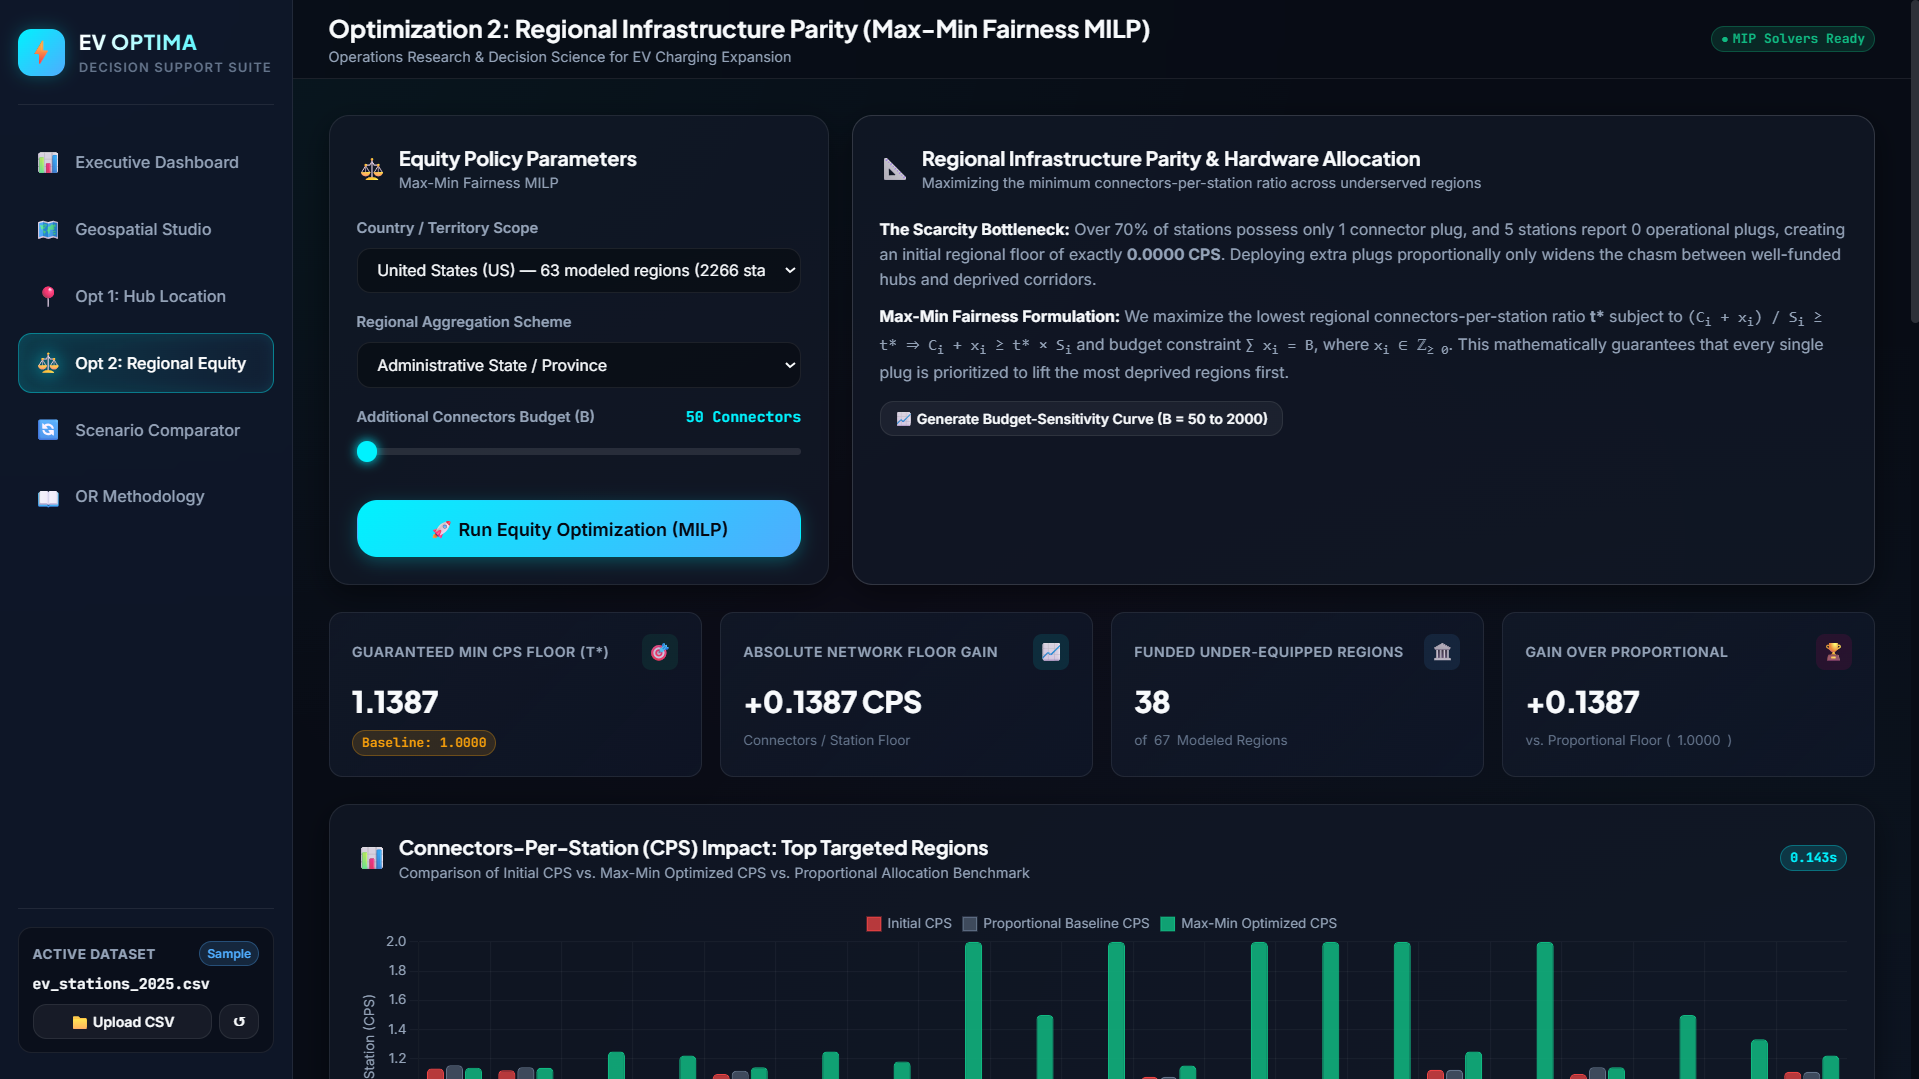
\includegraphics[width=\textwidth,height=0.82\textheight,keepaspectratio]{images/Optimization2.png}
    \end{column}
    \begin{column}{0.36\textwidth}
      \textbf{\color{Teal}US Equity Metrics ($B=50$)}
      \begin{itemize}\setlength{\itemsep}{0.22cm}
        \item \textbf{Floor Lift:} Minimum regional ratio rises from \textbf{1.0000 to 1.1387 CPS} (+0.1387 gain).
        \item \textbf{Targeted Funding:} Exactly \textbf{38 of 67 US regions} receive additional plugs.
        \item \textbf{vs. Proportional:} Naive allocation gives small states 0 plugs, leaving floor at 1.0000.
      \end{itemize}
    \end{column}
  \end{columns}
\end{frame}

% ---------------------------------------------------------
% SLIDE 17: RESULTS - OPTIMIZATION 2 CPS BAR GRAPH
% ---------------------------------------------------------
\begin{frame}{Results: Regional CPS Equity Distribution}
  \begin{columns}[c]
    \begin{column}{0.62\textwidth}
      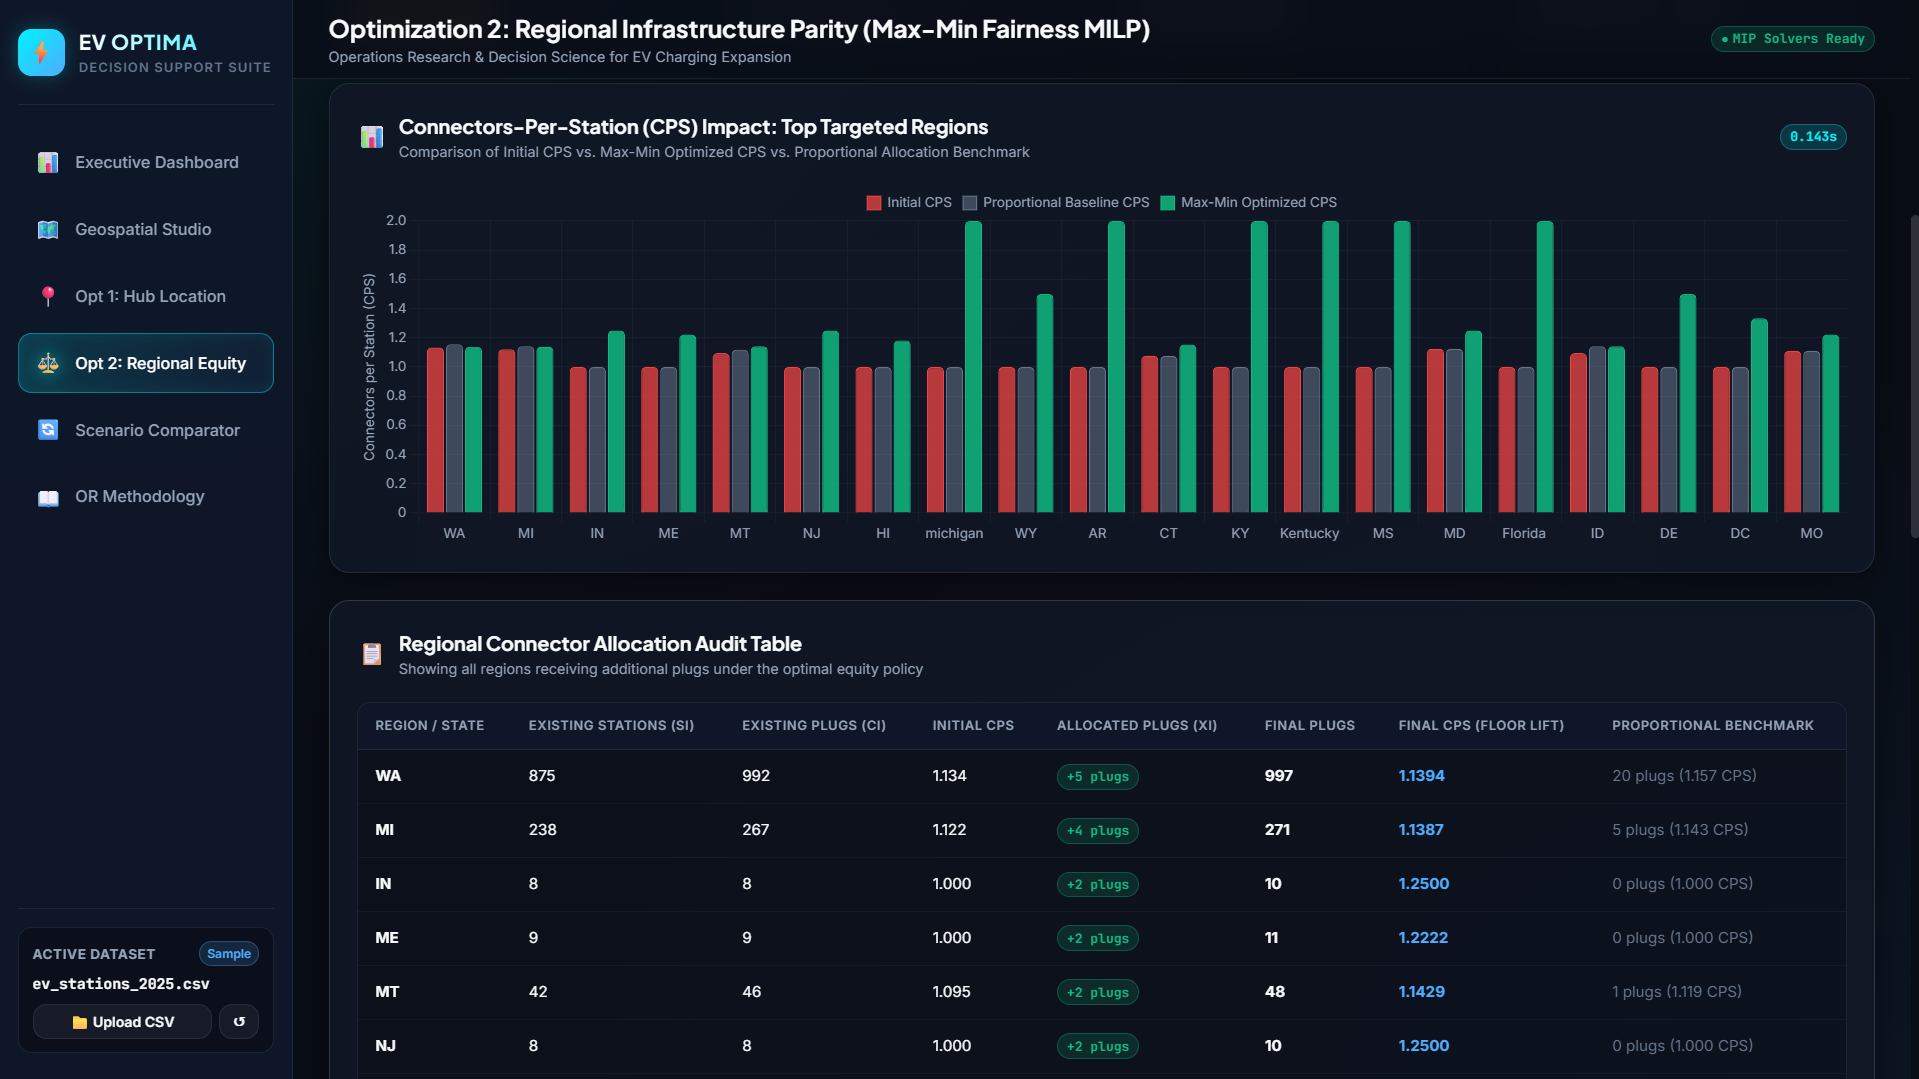
\includegraphics[width=\textwidth,height=0.82\textheight,keepaspectratio]{images/Optimization2_CPS.png}
    \end{column}
    \begin{column}{0.36\textwidth}
      \textbf{\color{Navy}Distribution Takeaways}
      \begin{itemize}\setlength{\itemsep}{0.22cm}
        \item \textbf{Leveling Effect:} Green bars compress lagging states up to $\ge 1.1387\text{ CPS}$.
        \item \textbf{Small State Support:} IN, ME, and NJ receive +2 plugs each (reaching 1.25 CPS).
        \item \textbf{Budget Met:} All 50 plugs integer-allocated to resolve regional deficits.
      \end{itemize}
    \end{column}
  \end{columns}
\end{frame}

% ---------------------------------------------------------
% SLIDE 19: CONCLUSION (5 SINGLE-LINE POINTS)
% ---------------------------------------------------------
\begin{frame}{Conclusion}
  \vspace{0.3cm}
  \begin{itemize}\setlength{\itemsep}{0.42cm}
    \item \textbf{Data-Driven Precision:} Operations Research mathematically transforms EV infrastructure planning from ad-hoc guesswork into provably optimal engineering.
    \item \textbf{Macro Capital Efficiency:} Siting just 10 strategic brownfield charging hubs covers over 33\% of the global network, outperforming random placement by 581\% ($15.94\sigma$).
    \item \textbf{Brownfield Cost Optimization:} Upgrading existing charging sites preserves capital by leveraging established electrical grid interconnects, road access, and permits.
    \item \textbf{Territorial Fairness Guaranteed:} Max-Min fair connector allocation eliminates regional charging deserts, lifting underserved jurisdictional floors to guaranteed baselines.
    \item \textbf{Interactive Decision Support:} The full-stack decision platform allows policymakers and private operators to simulate realistic planning scenarios in under one second.
  \end{itemize}
\end{frame}

% ---------------------------------------------------------
% SLIDE 20: THANK YOU SLIDE (JUST THANK YOU)
% ---------------------------------------------------------
\begin{frame}[plain]
  \begin{tikzpicture}[remember picture,overlay]
    \fill[Navy] (current page.north west) rectangle (current page.south east);
  \end{tikzpicture}
  \centering
  \vspace{3.0cm}
  {\Huge\bfseries\color{white} Thank You\par}
\end{frame}

\end{document}